\documentclass[
%% TIKZ_CLASSOPTION %%
tikz
]{standalone}
\usepackage{amsmath}
\usetikzlibrary{matrix}
%% EXTRA_TIKZ_PREAMBLE_CODE %%
\begin{document}
%% TIKZ_CODE %%
   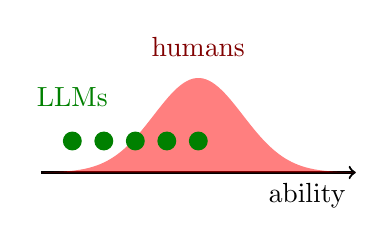
\begin{tikzpicture}[scale=4]
   \draw[thick,->] (0,0)  -- (1,0) node[anchor=north east]{ability};
   \fill[red,opacity=0.5,thick,domain=0:1,samples=100] (0,0)-- plot(\x,{0.3*exp(-((\x-0.5)^2)/(0.2^2))}) -- (1,0) -- cycle;
   \node[red!50!black] at (.5,.4) {humans};

   \fill[green!50!black] (.1,.1) circle(0.03);
   \fill[green!50!black] (.2,.1) circle(0.03);
   \fill[green!50!black] (.3,.1) circle(0.03);
   \fill[green!50!black] (.4,.1) circle(0.03);
   \fill[green!50!black] (.5,.1) circle(0.03);
   \node[green!50!black,below] at (.1,.3) {LLMs};
\end{tikzpicture}
\end{document}
